% Chapter Template

\chapter{PubSeq Web Service} % Main chapter title

\label{Chapter6} % Change X to a consecutive number; for referencing this chapter elsewhere, use \ref{ChapterX}

\lhead{Chapter 6. \emph{PubSeq Web Service}} % Change X to a consecutive number; this is for the header on each page - perhaps a shortened title

In this chapter we address the third question posed in Section \ref{sec:Chap3Intro}: \textit{How the user is going to \textit{retreive} the data?}. First, we would define our Virtual Machine environment on which our system runs. We would then delve into the structure of our Node.js server, how it initializes a web page and how it would interact with our service. Finally we would see how a user would generally use PubSeq, from giving in sequence to receiving and navigating over the results.


%----------------------------------------------------------------------------------------
%	SECTION 1
%----------------------------------------------------------------------------------------
\section{PubSeq Virtual Machine}

Two main components of PubSeq: PubSeq Solr Index and PubSeq Node.js server lay within a defined Virtual Machine within Rostlab internal network. Once a user opens a path that is directed to our Solr web server, the request would first land on Rostlab.org web server. Rostlab.org web server would then forward this request further to our PubSeq Node.js web server. The service would then render the page that the user will use to communicate with our server. All requests and responses between web page and PubSeq Node.js server would be proxied through Rostlab.org apache server (see Figure \ref{fig:PubSeqVM}). Our Virtual Machine is accessible internally via an assigned IP address and could also access other components within Rostlab network such as the SunGrid Engine (SGE). This IP address is however, not accessible from outside world. This guarantees that our Virtual Machine, particularly the Solr Index, which communicate via HTTP, couldn't be accessed from outside the world and thus prevents an unwanted disruption such as database injection.

To further ensure consistency of our Virtual Machine, we create a snapshot of the the VM once every day. Out of daily snapshots, we would keep the snapshots form the last two days. This way, we can always roll back our VM in case something would happen on it.

\begin{figure}[htbp]
    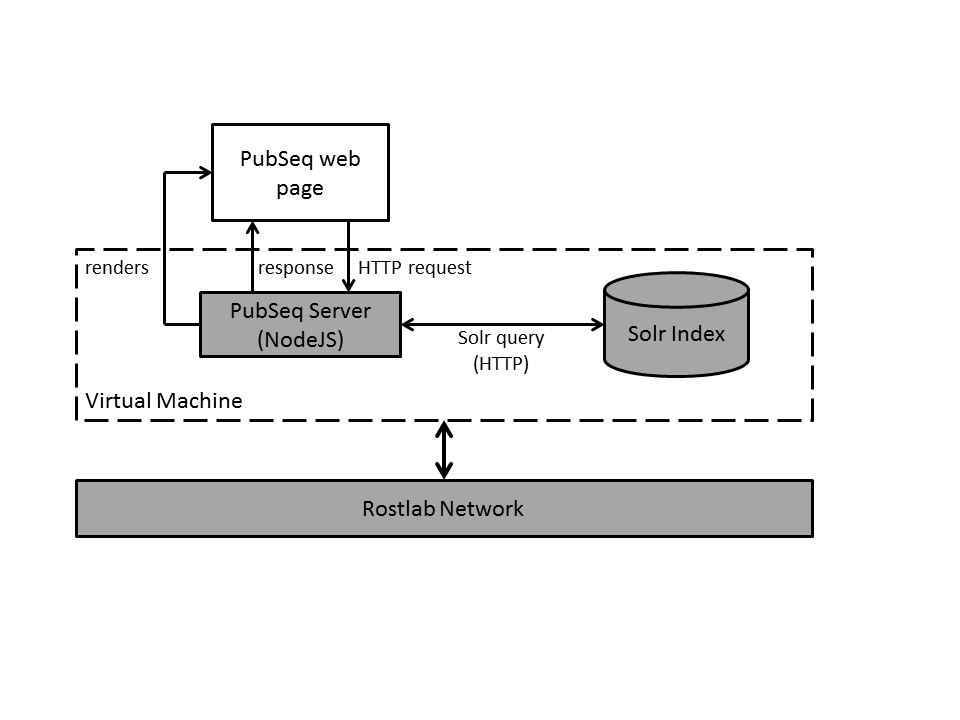
\includegraphics[width=6in]{Figures/pubseq_vm.png}
    \rule{35em}{0.5pt}
  \caption[Schematic representation of PubSeq systems with the Virtual Machine environment shown.]{Schematic representation of PubSeq systems with the Virtual Machine environment shown. Here we see the relative position and content of our Virtual Machine within Rostlab local area network (LAN). Rostlab SunGrid Engine (SGE) cluster and most other constituents within Rostlab networks are accessible from Virtual Machine \textit{vice versa}.}
  \label{fig:PubSeqVM}
\end{figure}

\subsection{VM Specifications}

Following are the specifications of our Virtual Machine:

\textbf{Kernel:}

\begin{lstlisting}[breaklines]
Linux pubseq-web.rostclust 3.16.0-4-amd64 #1 SMP Debian 3.16.7-ckt11-1 (2015-05-24) x86_64 GNU/Linux
\end{lstlisting}

\textbf{Distribution:}
\begin{lstlisting}[breaklines]
Disribution:		Debian GNU/Linux 8.1 (jessie)
Release:		8.1
Codename:		jessie
\end{lstlisting}


\textbf{Processors:}
\begin{lstlisting}[breaklines]
Core:			1
CPU MHz:		2599.998
BogoMIPS:		5199.99
CPU RAM GB:		6
Architecture:		x86_64
\end{lstlisting}

Here we see that our VM has relatively low RAM and number of core compared to other constituents within the network \footnote{One typical node in Rostlab's cluster has about 32 GB RAM and 12 cores}. The reason for this is because computationally expensive computations within our system, PubSeq Tagging Pipeline and BLAST, are always delegated to Rostlab SunGrid Engine (SGE). The two components that persistently run on our VM, Node.js Server and Solr, don't take a lot of memory and computing power. A lightweight Solr instance usually takes about 500 MB memory to run -- in our case, we only limit our memory use use to 1 GB RAM. Node.js is elastically implemented -- that is, it only requires memory that it needs. This means that in a given time, when there is no request, memory usage is nothing but negligible.

%----------------------------------------------------------------------------------------
%	SECTION 2
%----------------------------------------------------------------------------------------
\section{PubSeq Web Server}

In this project, we used Node.js for server side networking and scripting purpose. Node.js is a runtime environment for applications written in JavaScript. Unlike conventional JavaScript which runs on webpage within web browser engine, Node.js enables JavaScript application to run in command line environment. It provides event-driven and lock-free I/O API \citep{nodejs}, which makes it suitable for real-time web application. Node.js achieves this by utilizing the so-called Event Loop (see Figure \ref{fig:NodeJS}). 


Node.js is based on V8 Virtual Machine, which unlike other more traditional JavaScript VM, compiles JavaScript to native machine code instead of interpreting the code and then compiling it \citep{v8javascript}. All these characteristics make Node.js suitable for running a web application that handles thousands of concurrent connections with minimal overhead possible. We also chose Node.js as our web server environment since it allows compatibility with regard to data communication between web server and client, since native JSON would be used to communicate between the two. Specifically for Node.js, we use Express framework to implement our server, which is the most commonly used web service framework in Node.js \citep{expressjs}.

\begin{figure}[htbp]
    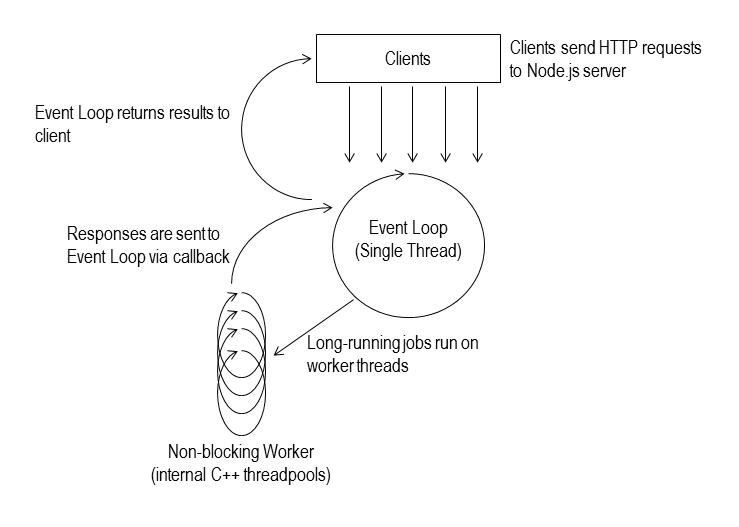
\includegraphics[width=6in]{Figures/nodejs.png}
    \rule{35em}{0.5pt}
  \caption[Schema of Node.js's Processing Model.]{Node.js internal processing model. Upon the arrival of HTTP request in Node.js server, Event Loop, which is implemented as single thread, passes the request onto worker threads while also adding callback onto its stack. Upon finishing submitted job, callback function will be called to notify Event Loop. It would then return job's results to the requesting client. By avoiding spawning thread for every request, Node.js avoids the overhead that could occur in server that handles thousands of request in a given time. This makes it appropriate for multi-users web application. Figure adopted from (Stannard, 2011 \citep{stannard2011intro}) with modifications.}
  \label{fig:NodeJS}
\end{figure}

\subsection{Components}

There are two main components in our Node.js server: \textbf{app.js} and web page files.

\textbf{app.js}\footnote{See Appendix \ref{sec:AppJSPath} for the paht to app.js within the repository.} is the main entry in our server. It contains components that are needed to make the server running such as:

\begin{itemize}
\item Express.js application definition and initiation \footnote{See \href{http://expressjs.com/4x/api.html}{\texttt{http://expressjs.com/4x/api.html}} (accessed 26/08/2015) for Express.js API.}.
\item HTML rendering engine definition (see \textbf{Web Page Files} bellow).
\item Additional prototypical String functions such as hash code creating function  and \texttt{startsWith()} \footnote{Note that \texttt{startsWith()} will be implemented in upcoming ECMAScript 2015 (ES6) Standard, see \href{https://developer.mozilla.org/en/docs/Web/JavaScript/Reference/Global_Objects/String/startsWith}{\texttt{https://developer.mozilla.org/en/docs/Web/JavaScript/Reference/Global\_Objects/String/startsWith}} (accessed 26/08/2015).}
\item \texttt{GET}, \texttt{POST} handlers for each of available pages, if such method is defined within the page.
\item Several utility functions.
\end{itemize}

\textbf{Web Page Files} consist of pages that are available within the web application environment. Each page is written in Jade syntax, which makes it easier for user to write complex HTML file \footnote{\href{http://naltatis.github.io/jade-syntax-docs/}{\texttt{http://naltatis.github.io/jade-syntax-docs/}, accessed 26/06/2015.}}. Upon \texttt{GET} request for a page, \textbf{app.js} would render the page file using the HTML rendering engine for jade. This engine would parse the \texttt{.jade} file and create proper HTML file, which would then be returned to client.

\subsection{index.html}

Of most importance is the \textbf{index.html} (which was avaiable as \textbf{index.jade} prior rendering process) among web pages that are avaiable within the web interface environment. The web page contains the query interface that would communicate.